\documentclass{article}
\usepackage{setspace}
\usepackage[utf8]{inputenc}
\usepackage{natbib}
\usepackage{url}
\usepackage{indentfirst} 
\usepackage{hyperref}
\usepackage{xcolor}
\usepackage{float}

\usepackage{booktabs}
\usepackage{longtable}
\usepackage{array}
\usepackage{multirow}
\usepackage{wrapfig}
\usepackage{float}
\usepackage{colortbl}
\usepackage{pdflscape}
\usepackage{tabu}
\usepackage{threeparttable}
\usepackage{threeparttablex}
\usepackage[normalem]{ulem}
\usepackage[utf8]{inputenc}
\usepackage{makecell}
\usepackage{xcolor}

\usepackage{graphicx}
\graphicspath{ {figures/} }

\title{Text Analysis of \emph{Hamilton}}
\author{Nathan Schor}
\date{March 13, 2022}

\doublespacing
\begin{document}

\maketitle
\begin{singlespace}
\tableofcontents
\end{singlespace}

\section{Introduction}

The purpose of this research is apply natural language processing (NLP) to the lyrics of the musical \emph{Hamilton}. We construct an ontology for \emph{Hamilton}. As part of the analysis, we experiment with three different sources of stop words, four different sentiment lexicons, and tokenizing at the word vs. sentence level. Term frequency-inverse document frequency (\emph{tf-idf}) is used to identify the most important terms for each character, a topic model is created to see if it can identify characters based on phrases most likely to belong to them, and we build a chat bot that can answer general questions about the musical and our analysis. We begin by building an ontology. Next, we examine how sentiment changes throughout the musical. Next, we use \emph{tf-idf} to identify the most important word for each speaker. After, we see if the topic model is able to identify the speaker based on their words. Lastly, we develop a chat bot that is able to answer questions on a corpus that contains \emph{Hamilton's} Wikipedia page augmented with results from this analysis. 

Using \cite{Silge2022}




\section{Literature Review}

\section{Data}

\subsection{Corpus}

The main dataset is obtained from the website \cite{Kaggle2019}. It contains the entirety of the musical in a csv file with 3,634 rows and 3 columns. The \emph{Lines} column gives the line that is spoken. The \emph{Speaker} column gives the names of the people speaking (there can be more than one character singing at the same time). \emph{Title} gives the name of the song. 5 random rows of the data are shown in Table \ref{tab:example}. The main corpus for the chat bot is \cite{Wiki}.

\begin{table}
\caption{Five rows from the \emph{Hamilton} dataset.}
\label{tab:example}

\begin{tabular}{r|l|l|l}
\hline
entry & title & speaker & lines\\
\hline
1 & The Election of 1800 & JEFFERSON & 'cuz I'm the President. Hey, Burr, when you see Hamilton, thank him for the endorsement\\
\hline
2 & Blow Us All Away & PHILIP & I came to ask you for advice. This is my very first duel\\
\hline
3 & It's Quiet Uptown & HAMILTON & I take the children to church on Sunday\\
\hline
4 & Satisfied & ANGELICA & Have to be na<ef>ve to set that aside\\
\hline
5 & Right Hand Man & WASHINGTON & But the elephant is in the room\\
\hline
\end{tabular}

\end{table}

\subsection{Stop Words}

Three sources are used to obtain the list of stop words. They are the SMART lexicon from \cite{Lewis2004}, snowball from \cite{snowball}, and onix. SMART contains 571 stop words, snowball has 174 stop words, and onix has 404 stop words.

\subsection{Sentiment}

Three lexicons are used to obtain sentiment. They are the AFINN dataset from \cite{nielsen11}, the nrc dataset from INSERT HERE, and the bing dataset from INSERT HERE.

AFINN assigns words an integer value in $\{-5, -4, ..., 4, 5\}$ with -5 having the most negative sentiment and 5 having the most positive sentiment. Swear words/insults have -5, words like "superb" or "breathtaking" are 5, and "some kind" is 0. There are 2,477 terms. 

The nrc dataset assigns each of its 13,875 words to 1 of 8 emotional categories. For the purpose of this analysis, only words in the "positive" or "negative" emotion category are retained. 

The only sentiment dataset ready for off-the-shelf use is the bing dataset. It classifies 6,786 terms as having either positive sentiment or negative sentiment. It is worth noting that roughly 70\% of the terms are negative, so negative sentiment words are over-represented. 


\section{Research Design and Modeling Methods}

\subsection{Ontology}

I began by thinking about which aspects of \emph{Hamilton} would be interesting to analyze using NLP tools. To structure my thinking, I constructed an ontology. The key pieces of the musical are its songs and actors. Within songs, I was curious how the mood changed throughout the duration of the play. For the actors, I was interested in analyzing whether were particular words or phrases could summarize a character's behavior. Figure \ref{fig:ontology} shows the ontology I created using INTERSET PROTEGE. It served as my starting point for which kind of NLP questions to tackle. 

\begin{figure}[h]
    \caption{Ontology for \emph{Hamilton}. \label{fig:ontology}}
    \centering
    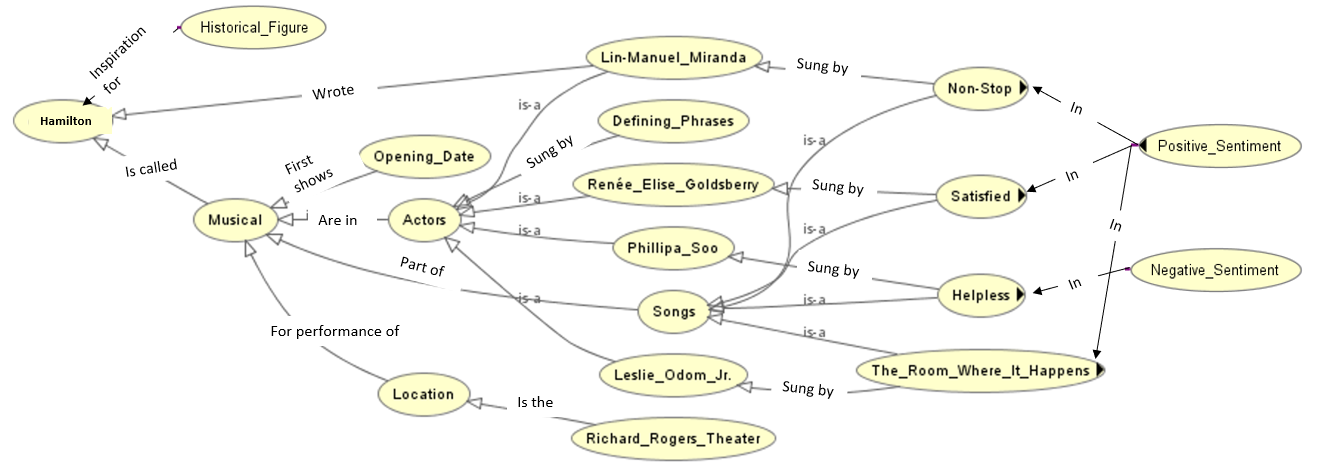
\includegraphics[width=0.7\paperwidth, scale=1.25]{ontology.png}
\end{figure}

The 4 main areas of investigation were analyzing mood via sentiment analysis, investigating the most important words for speakers using \emph{tf-idf}, seeing if we could ``uncover" the speaker using topic models, and creating a chat bot to answer general questions about the play as well as information from the first 3 parts. Each of these are discussed in turn.

\subsection{Sentiment Analysis}

The two questions for this section are how much does differing the source of word sentiment affect the "time series" of the play's sentiment, and which song \emph{s} has the greatest mood shift, defined as $max(Sentiment_{s} - Sentiment_{s - 1})$ for $s = \{2, 3, ..., S - 1, S\}$ ($s - 1$ is not defined for $s = 1$).

The \emph{Hamilton} lyrics were first tokenized into words and normalized to lower case. A song's sentiment was calculated as $Sentiment_{s} = \sum_{w = 1}^{W}w$ where \emph{W} is the total number of words in song \emph{s}. This approach has a few major limitations. One is that a song's sentiment is not necessarily the sum of its parts. For example, \emph{It's Quiet Uptown} starts off with the death of Hamilton's son and has very negative sentiment. The end of the song has a positive sentiment as Hamilton and Eliza rekindle their marriage. This simple counting fails to capture the mood shift that transpires during the song. Furthermore, tokenizing at the word level does not capture the impact of negative modifiers. For example, the sentence ``I was not happy with the show" should have negative sentiment, but the term ``happy" will count as positive sentiment.

The \emph{sentimentr} package helps to overcome some of these shortcomings. It tokenizes words as the sentence level rather than at the word level. This additional context can help to assign the correct overall sentiment to a sentence since its sentiment is not necessarily the sum of its individual tokens. 

\subsection{TF-IDF}
\label{section:tf-idf}

\emph{tf-idf} is comprised of two parts: term frequency \emph{tf} and inverse document frequency \emph{idf}. The idea is that "important" words are captured by the seemingly contradictory idea that important words are both frequent and rare. A word's term-frequency is the number of times the word appears in the document divided by total number of words in the document (this is a way to control for the size of the document). The word's inverse document frequency is the natural logarithm of the number of documents in the corpus divided by the number of documents in the corpus that contain that word. The idea is that a common word such as "the" will have a high term frequency, but is not necessarily important or informative. However, "the" will have a low inverse document frequency because it is likely that every single document in the corpus will contain the word "the". Using \emph{tf-idf} helps to balance these two by multiplying them together. Thus, a word with a high \emph{tf-idf} both occurs frequently in a given document, but is rare in the corpus as a whole. 

We use \emph{tf-idf} as the metric to determine which are the most important words for a given speaker. For this analysis, we define a speaker as a character who has 10 or more solo lines. In the musical, many characters are singing simultaneously. In the dataset, it is challenging to parse out which words are attributed to each speaker since a list of speakers can be given for the same line. Thus we only look at lines where a speaker was the only singer in this analysis (which introduces some bias since there could be important information lost). 

\subsection{Topic Modeling}

Topic modeling is an unsupervised learning method that seeks to group documents into k similar documents, or topics. Since it is unsupervised, there is no loss function that can be used to optimize k since we do not have a "true" value. One of the most common algorithms for topic modeling is Latent Dirichlet Allocation (LDA) that treaks every document as being comprised of multiple topics, and every topic being comprised of multiple words. LDA estimates both of these quantities simultaneously. In this project, we look at the solo lines song by Hamilton, Eliza, and Washington. We see if we can recover words that uniquely identify these characters. Thus, the true k is 3, and we see if the topic model is able to identify the 3 "topics".

\subsection{Chat Bot}

The final portion of this project creates a chat bot that can answer questions about the \emph{Hamilton} Wikipedia page and on the previous 3 subsections. We do this using the following NLP pipeline:
\begin{singlespace}
\begin{enumerate}
 \item Convert all strings to lower case
 \item Tokenize the data at the sentence level
 \item Perform lemmitization
 \item Calculate the \emph{tf-idf} for each token
 \item Return the entry from the corpus that has the largest cosine similarity with the query. 
\end{enumerate}
\end{singlespace}

Cosine similarity measures the "distance" between two quantities by computing the angle $\theta$ between them. Each token is plotted as a vector using its \emph{tf-idf}. As we see from the formula $cos(\theta_{token1, token2}) = \frac {token1 \cdot token2}{||token1|| \cdot ||token2||}$, the cosine similarity for two vectors is between -1 and 1. Two identical vectors will have a cosine similarity of 1. The chat bot only returns results for queries that have a cosine similarity of at least 0 with another sentence in the corpus. 

\section{Results}

Figure \ref{fig:sentiment} shows how sentiment changes over the course of the musical. The song number (1-45) is displayed on the x-axis. The y-axis shows the sentiment. Notice that the scale between sentiment datasets can differ; for example, sentiment for the AFINN dataset is between -50 and 50, while sentiment from \emph{sentimentr} is between -10 and 20. The important aspect is not the absolute value of the sentiment, but the direction (positive or negative) and a song's sentiment value relative to other songs using the same sentiment dataset. 

\begin{figure}[h]
    \caption{Sentiment analysis by sentiment dictionary. \label{fig:sentiment}}
    \centering
    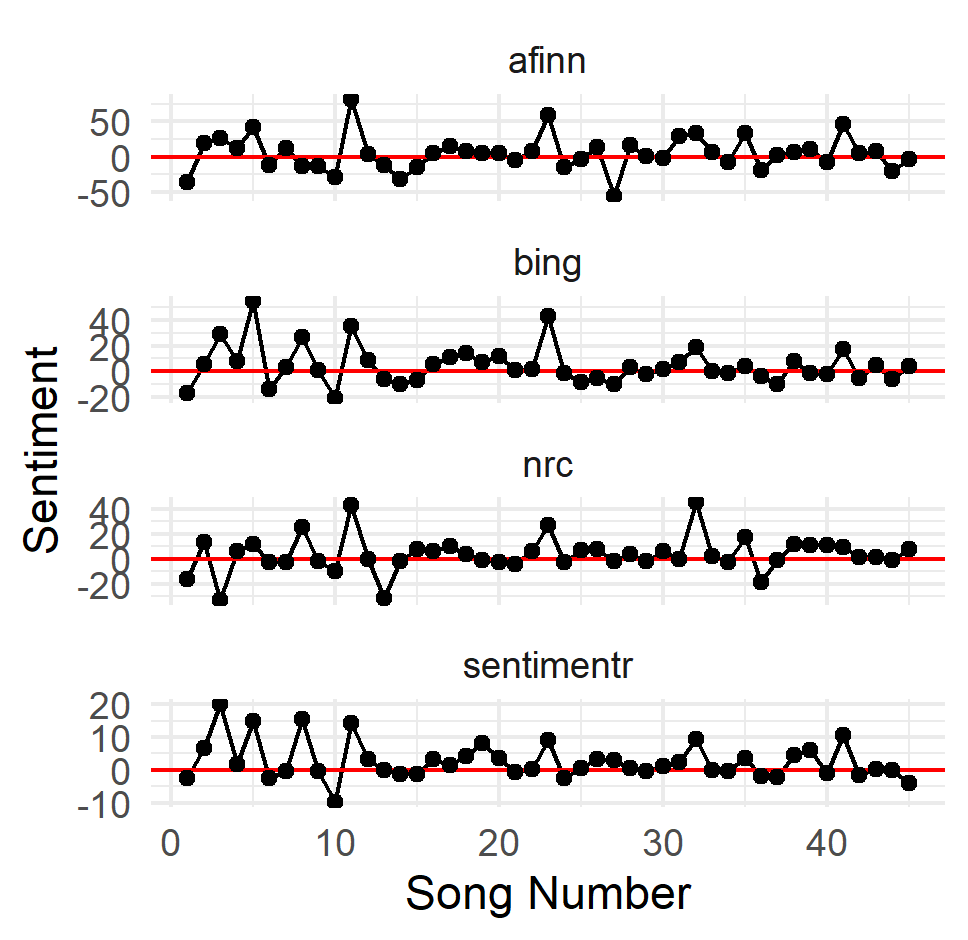
\includegraphics[width=0.5\paperwidth, scale=1]{sentiment_by_stopwords.png}
\end{figure}

Table \ref{tab:tfidf} displays the word with the largest \emph{tf-idf} for each speaker. The SMART, snowball, and onix columns show had those respective stop word dictionaries applied to the data. The "All Lexicons" column had all 3 stop word dictionaries applied, and "All Words" did not remove any stop words. Speakers who appear multiple times had ties for their most important word in at least 1 of the 5 processing coluns. For example, Lafayette's most important word when any kind of stop word processing is used is "onarchy", but without stop word removal his most important word is "oui". Similarly to section \ref{section:tf-idf}, a speaker is defined as someone who is the only person singing a given line. This removes ambiguity over which speaker is singing a line. 

\begin{table}
\caption{Speaker \emph{tf-idf} by stop word lexicon.}
\label{tab:tfidf}

\begin{tabular}{r|l|l|l|l|l|l}
\hline
\textbf{Entry} & \textbf{Speaker} & \textbf{SMART} & \textbf{snowball} & \textbf{onix} & \textbf{All Lexicons} & \textbf{All Words}\\
\hline
1 & Angelica & satisfied & satisfied & satisfied & satisfied & satisfied\\
\hline
2 & Burr & room & room & immigrant & immigrant & room\\
\hline
3 & Company & number & number & aaaah & aaaah & number\\
\hline
4 & Eliza & huit & enough & look & huit & enough\\
\hline
5 & Eliza & huit & enough & look & sept & enough\\
\hline
6 & Ensemble & buck & buck & buck & buck & buck\\
\hline
7 & Hamilton & sir & sir & sir & sir & i\\
\hline
8 & Jefferson & what'd & what'd & what'd & what'd & what'd\\
\hline
9 & Lafayette & onarchy & onarchy & onarchy & onarchy & onarchy\\
\hline
10 & Lafayette & onarchy & onarchy & onarchy & onarchy & oui\\
\hline
11 & Laurens & colonies & colonies & colonies & colonies & colonies\\
\hline
12 & Lee & crisis & crisis & crisis & crisis & crisis\\
\hline
13 & Madison & size & size & size & size & size\\
\hline
14 & Maria & sir & yes & yes & sir & yes\\
\hline
15 & Men & satisfied & satisfied & satisfied & satisfied & satisfied\\
\hline
16 & Mulligan & hercules & hercules & hercules & hercules & hercules\\
\hline
17 & Mulligan & hercules & hercules & hercules & hercules & lovin\\
\hline
18 & Philip & deux & deux & deux & deux & deux\\
\hline
19 & Philip & deux & deux & deux & deux & huit\\
\hline
20 & Seabury & heed & heed & heed & heed & heed\\
\hline
21 & Seabury & heed & heed & heed & heed & interests\\
\hline
22 & Washington & goodbye & goodbye & goodbye & goodbye & goodbye\\
\hline
23 & Women & helpless & helpless & helpless & helpless & helpless\\
\hline
\end{tabular}

\end{table}

In Figure \ref{fig:topic_model} we have a topic model. The y-axis shows 10 terms for each topic. On the x-axis is $\beta$, which is the probability that the given term one generated from their assigned topic. For example, the term "sir" has a .02 probability of being generated from topic 1. Notice that terms (such as "sir" can overlap between topics. This seems reasonable given that all of the "topics" are speakers in the same play.

\begin{figure}[h]
    \caption{Topic model generated with lines from Hamilton, Washington, and Eliza. \label{fig:topic_model}}
    \centering
    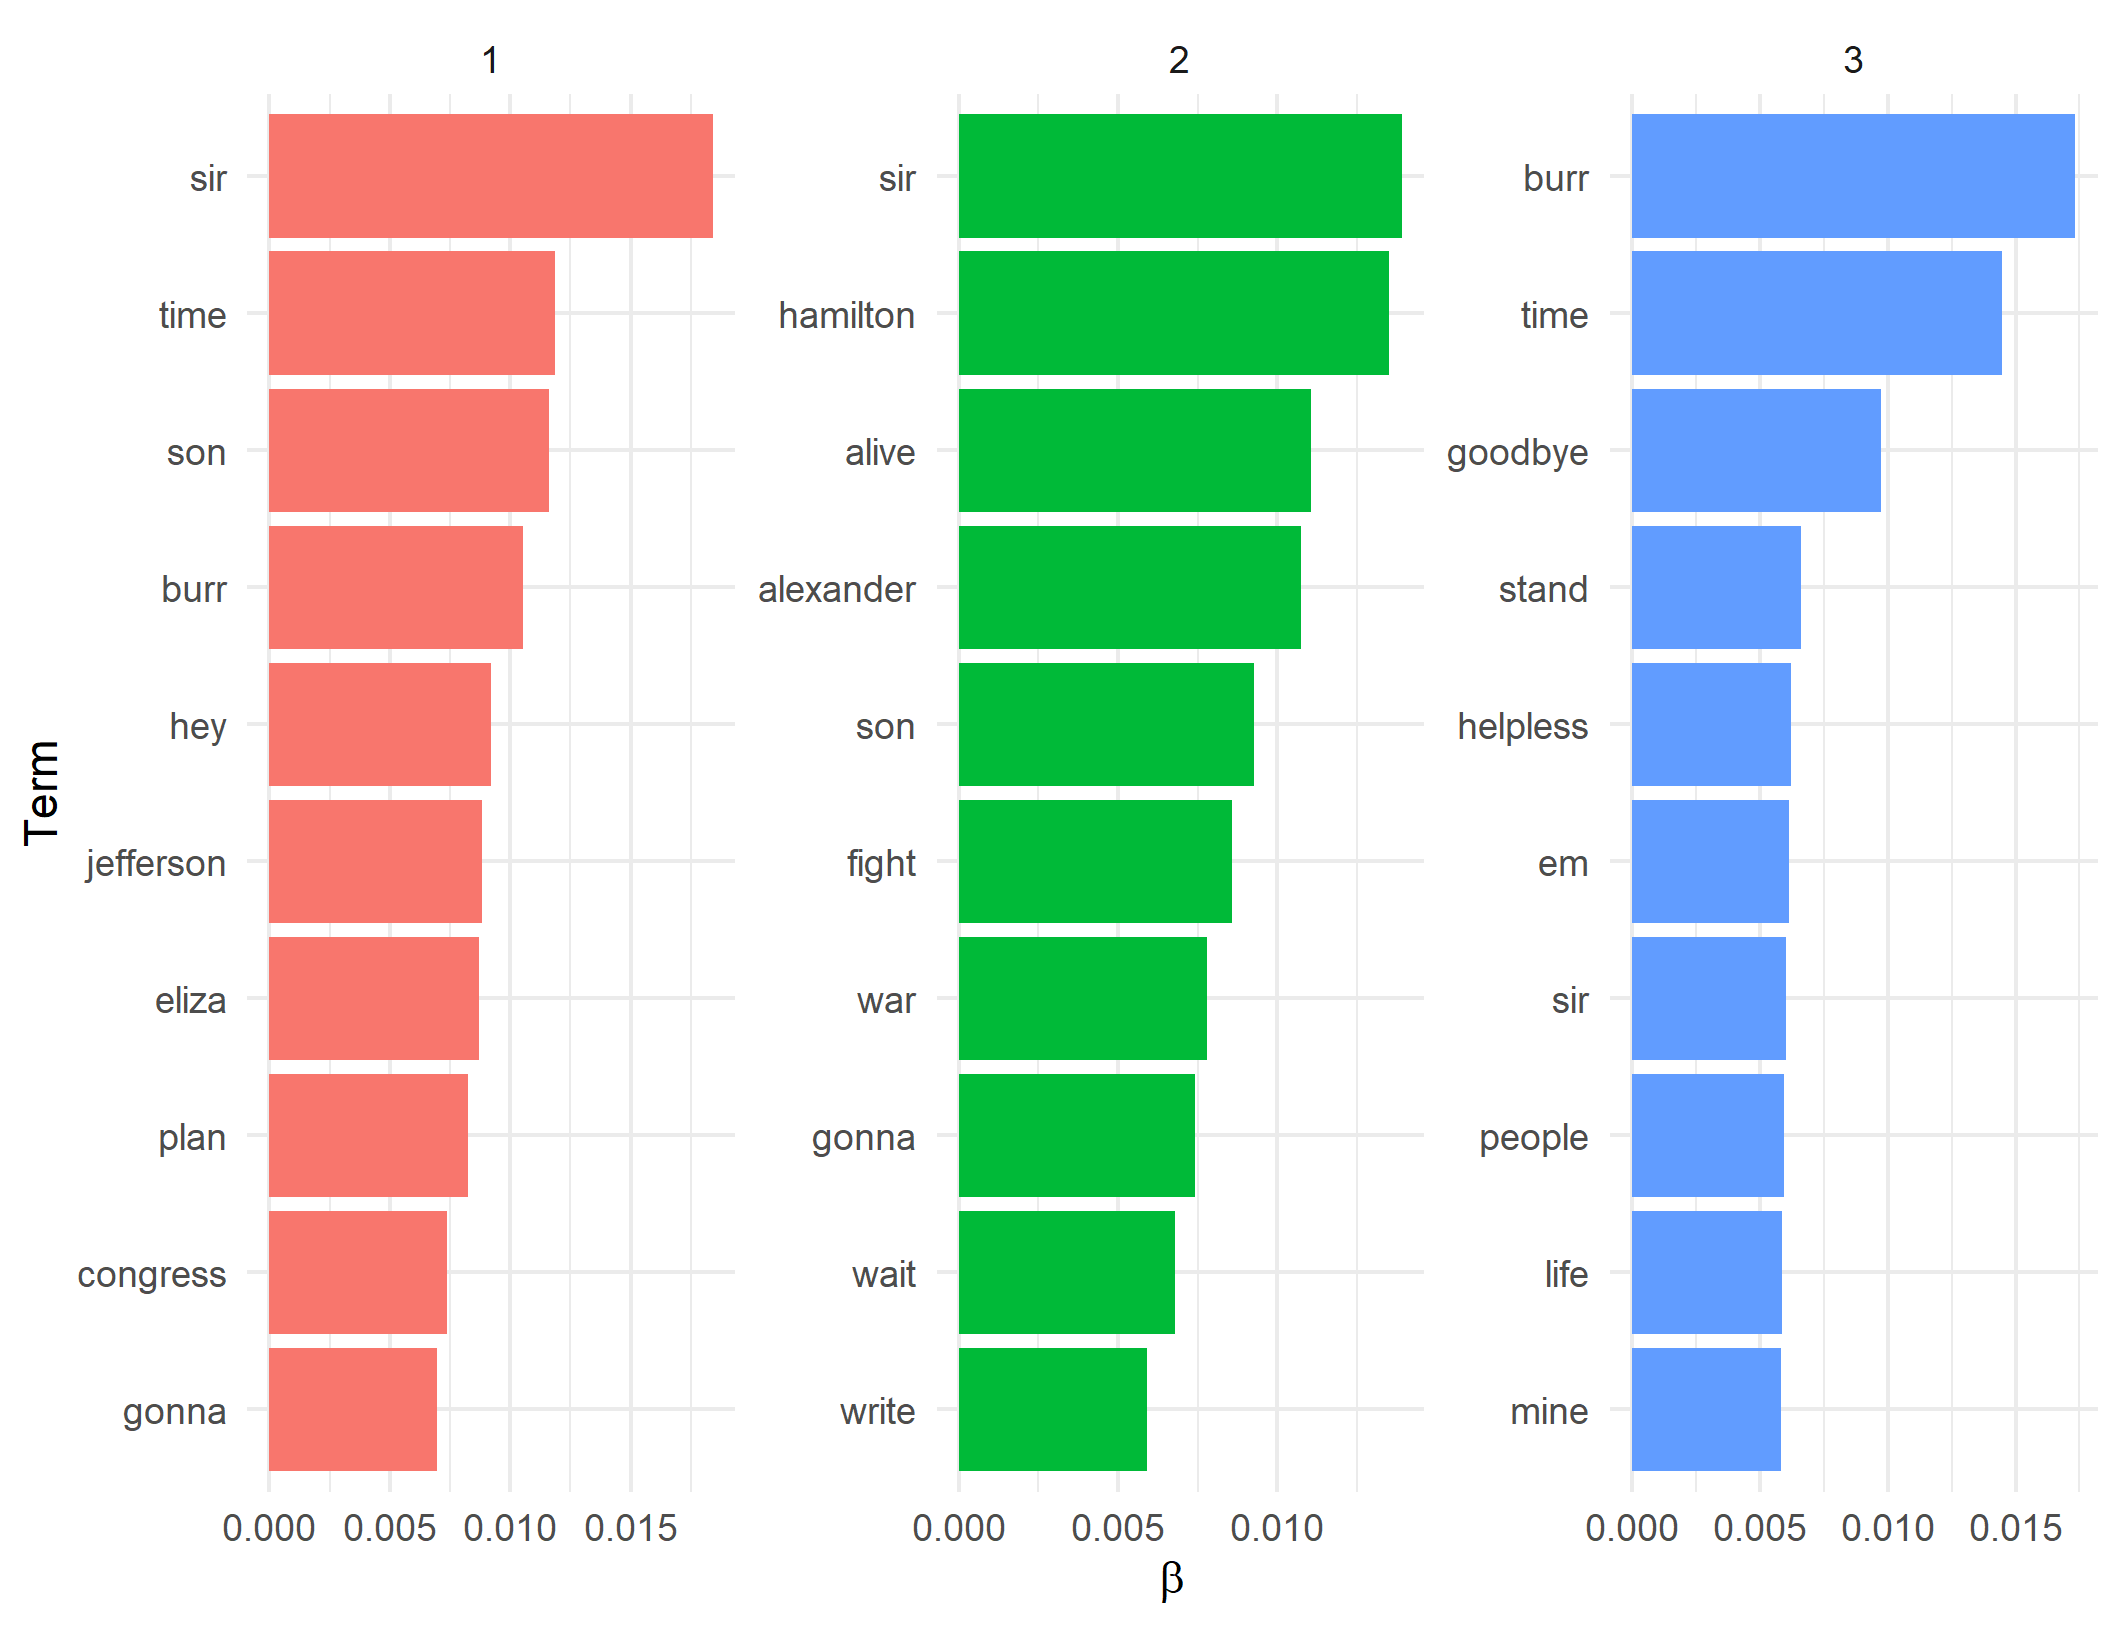
\includegraphics[width=0.7\paperwidth]{topic_model.png}
\end{figure}

An example of the chat bot's output is show in Figure \ref{fig:chat_bot}. The text that is generated at the beginning of each conversation ("\emph{Don't Throw Away Your Shot to ask me questions about Hamilton! Type them in the box below:}") is italicized. The user's question is in \textbf{bold} and the chat bot's response is colored. A \textcolor{green}{green} response indicates that the chat bot answered well, a \textcolor{yellow}{yellow} response means that the response was on the right track but not quite correct, and \textcolor{red}{red} means the response was unsatisfactory. 

\begin{figure}[h]
    \caption{Example output from 5 queries fed to the chat bot. \label{fig:chat_bot}}
    \centering
    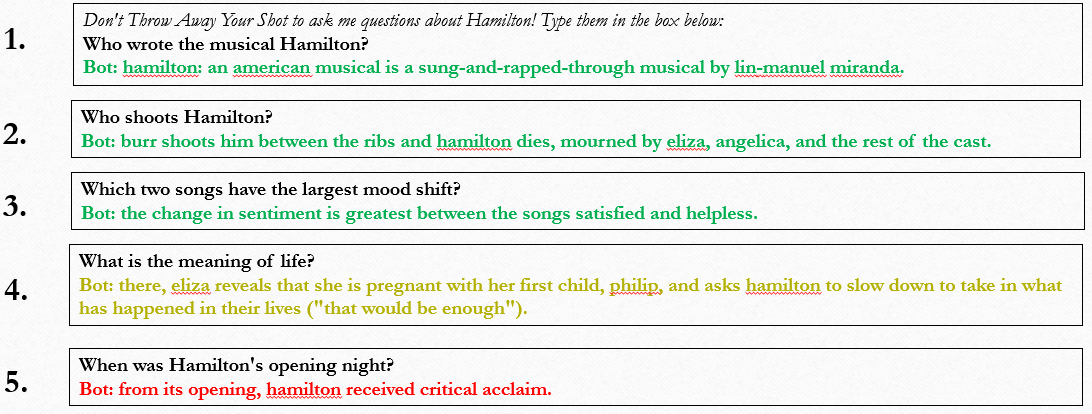
\includegraphics[width=0.7\paperwidth]{chat_bot_output.png}
\end{figure}


\section{Analysis and Interpretation}

\subsection{Sentiment}

Thoughtfully selecting a sentiment dataset is important to the results. Each of the sentiments in Figure \ref{fig:sentiment} have large swings in sentiment up until song 11 (\emph{Satisfied}), after which the sentiment has lower variance. All of graphs identify \emph{Satisfied} as one of the most positive songs and \emph{Helpless} (song 10) as one of the most negative songs and show that Act I ends on an extremely positive note with \emph{Non-Stop} (song 23). However, AFINN and \emph{sentimentr} identify the final song as having negative sentiment while nrc and bing classify the song as overall positive. There are a number of songs where the datasets diverge in classifying the song's valence. Thus, sentiment is conditional on the dataset used.

\subsection{TF-IDF}

Similarly, it is important to carefully construct a list of stop words that are \emph{corpus specific}. For example, in Figure \ref{tab:tfidf} "sir" could reasonably be considered a stop word. It is interesting how changing the stop word preprocessing step affects the speaker's most important word. For example, Burr's most important words are "room" and "immigrant". "room" is an inward looking term for Burr, reflecting his desire to be in the "room" when decisions are being made and to have a seat at the table. "immigrant" is an outward looking term, reflecting his complicated relationship with Hamitlon--who Burr often refers to as the "immigrant." It's also noteworthy that \emph{tf-idf} identifies the "catch phrase" for a number of the speakers: "satisfied" for Angelica, "goodbye" for Washington, "yes" for Maria Reynolds, and "enough" for Eliza.  

\subsection{Topic Model}

The topic model in Figure \ref{fig:topic_model} was able to produce reasonable terms for each of the three speakers from which the topics were generated (Hamilton, Eliza, and Washington). Topic 1 seems to be about Hamilton--Hamilton is fixated on the concept of time and speaks frequently with his son (Phillip), Jefferson, Burr, and Eliza. Topic 2 appears to identify Washington. Washington talks frequently with Hamilton and is heavily involved with the Revolutionary War and the fighting. To Hamilton's dismay, Washington refers to Hamilton as "son" (note that "son" appears in both the "Hamilton Topic" and the "Washington Topic" despite having a slightly different meaning). Eliza is the speaker identified in Topic 3. The term "helpless" is the title of one of her main songs and one of her catch phrases. She often speaks with Hamilton about "life" and unfortunately has to say "goodbye" to both her son Phillip and to Hamilton when they are each killed in duels. This topic modeling experiment illustrates that it has the potential to be used in situations where the number of topics is not known \emph{a priori} as a way of summarizing text.

\subsection{Chat Bot}

In Figure \ref{fig:chat_bot}, we see that the chat bot performs well on 3 queries, decently on 1 query, and poorly on the final query. A more sophisticated chat bot would be able to answer the question \textbf{"Who shoots Hamilton?"} with just the correct answer, "Burr", rather than providing all of the unnecessary context that is present in the Wikipedia document about the characters who mourn Hamilton. In query 3, we see that the chat bot correctly retrieves the relevant information for a query that is targeting the dataset augmented with the results from Figure \ref{fig:sentiment}. It seems plausible that a non-technical user would use the term "mood" rather than "sentiment", and we see that the chat bot has no problem retrieving the key sentence. 

Query 4 is the most interesting. In a literal sense, the query does not explicitly answer the user's question; the question does not ask about Eliza's pregnancy or her request to Hamilton. However, the chat bot does (perhaps unintentionally) offer a profound response to the age-old question: \emph{"What is the meaing of life?"}. The answer touches on the importance of family, as well as slowing down and taking things one at a time and being happy with what they do have instead of focusing on what they do not. This example illustrates that a chat bot which can only retrieve text rather than generate text certainly has limitations, it has the potential to use its corpus in unexpected ways to produce interesting results.

The last query highlights a limitation of the cosine similarity approach. The bot relies too heavily on the word "opening" and returns irrelevant results. A more sophisticated bot would understand that a necessary (but not sufficient) response would contain a time component e.g. "The show opened \textbf{6 years} ago. It would also identify phrases that serve the same purpose as "opening" such as "started", "began", "premiered", and "first shown". 

\section{Conclusions}

Often times, the most exciting parts of doing research are building models and generating informative tables and figures. However, the vast majority of time is spent in data acquisition, EDA, and data processing. This is especially true in NLP. Not only is each corpus different, but each use case with the same corpus is different. We need to take the time to make sure we truly understand the data we are working with so that we can feed useful information into our models. As the quote goes, "Garbage in, garbage out."

This project highlighted for me the importance of curating a corpus-specific stop word list. Off-the-shelf stop words can be a nice start, but the probability that the list was curated with your specific use case in mind is close to 0. The same is true for sentiment. 

The chat bot showed me that something useful can be built with even with a relatively little amount of code. However, the amount of work necessary to see incremental improvement increases sharply as the chat bot gets better and better. Alternative methods like BERT would likely have processed a better chat bot and is something I would like to explore in future work. 

\section{References}

\bibliography{references}
\bibliographystyle{apalike}


\end{document}